\documentclass{article}\usepackage[]{graphicx}\usepackage[]{color}
%% maxwidth is the original width if it is less than linewidth
%% otherwise use linewidth (to make sure the graphics do not exceed the margin)
\makeatletter
\def\maxwidth{ %
  \ifdim\Gin@nat@width>\linewidth
    \linewidth
  \else
    \Gin@nat@width
  \fi
}
\makeatother

\definecolor{fgcolor}{rgb}{0.345, 0.345, 0.345}
\newcommand{\hlnum}[1]{\textcolor[rgb]{0.686,0.059,0.569}{#1}}%
\newcommand{\hlstr}[1]{\textcolor[rgb]{0.192,0.494,0.8}{#1}}%
\newcommand{\hlcom}[1]{\textcolor[rgb]{0.678,0.584,0.686}{\textit{#1}}}%
\newcommand{\hlopt}[1]{\textcolor[rgb]{0,0,0}{#1}}%
\newcommand{\hlstd}[1]{\textcolor[rgb]{0.345,0.345,0.345}{#1}}%
\newcommand{\hlkwa}[1]{\textcolor[rgb]{0.161,0.373,0.58}{\textbf{#1}}}%
\newcommand{\hlkwb}[1]{\textcolor[rgb]{0.69,0.353,0.396}{#1}}%
\newcommand{\hlkwc}[1]{\textcolor[rgb]{0.333,0.667,0.333}{#1}}%
\newcommand{\hlkwd}[1]{\textcolor[rgb]{0.737,0.353,0.396}{\textbf{#1}}}%
\let\hlipl\hlkwb

\usepackage{framed}
\makeatletter
\newenvironment{kframe}{%
 \def\at@end@of@kframe{}%
 \ifinner\ifhmode%
  \def\at@end@of@kframe{\end{minipage}}%
  \begin{minipage}{\columnwidth}%
 \fi\fi%
 \def\FrameCommand##1{\hskip\@totalleftmargin \hskip-\fboxsep
 \colorbox{shadecolor}{##1}\hskip-\fboxsep
     % There is no \\@totalrightmargin, so:
     \hskip-\linewidth \hskip-\@totalleftmargin \hskip\columnwidth}%
 \MakeFramed {\advance\hsize-\width
   \@totalleftmargin\z@ \linewidth\hsize
   \@setminipage}}%
 {\par\unskip\endMakeFramed%
 \at@end@of@kframe}
\makeatother

\definecolor{shadecolor}{rgb}{.97, .97, .97}
\definecolor{messagecolor}{rgb}{0, 0, 0}
\definecolor{warningcolor}{rgb}{1, 0, 1}
\definecolor{errorcolor}{rgb}{1, 0, 0}
\newenvironment{knitrout}{}{} % an empty environment to be redefined in TeX

\usepackage{alltt}

\input{c:/aaaWork/zGnrlLatex/GnrlPreamble}
\usepackage{booktabs}
% Puts sections in TOC but does not number them
\setcounter{secnumdepth}{0}
\IfFileExists{upquote.sty}{\usepackage{upquote}}{}
\begin{document}
  \title{Course Level Assessment Report \\ MTH107 Statistical Concepts and Analysis}
  \author{\vspace{-12pt}Derek H. Ogle}
  \date{\vspace{-12pt}\today}
  \maketitle










\section{Course Information}
\subsubsection{Background}
\emph{Statistical Concepts and Analysis (MTH107)} is the entry-level statistics course at Northland College. Taught by instructors in the Mathematical Sciences program, the course is required by several majors in the Natural Resources, Environmental Sciences, and Social Responsibility departments and can also fulfill the ``quantitative reasoning'' requirement for the College's Connections program.

I have taught MTH107 since 1996, including 20 sections of MTH107 since 2010, the period for which this assessment document covers. Before the Winter 2016 term (listed as W16 in this analysis), my sections of MTH107 were lecture-based with minimal (approx. 25\%) class time devoted to ``hands-on'' in-class activities or experiences. Beginning in Winter 2016, the course was ``flipped'' such that the vast majority of class time was used for in-class activities and work, with minimal ``planned'' lectures for concepts that students typically struggled with and other ``lectures'' as questions warranted. For the ``flipped'' courses, student were asked to read a short amount of material (usually less than ten pages) and watch short videos (usually less than 30 minutes) to prepare for class. In class, students completed a short quiz (less than 10 minutes) to assess their preparedness of the material and then worked on a variety of exercises related to the material. Planned lectures usually used about half of the class period, with the remaining half devoted to in-class exercises. The flipped structure has been maintained through the most recent academic year, though several changes in the structure of the course content were implemented in Winter, 2018. The pedagogical change in Winter, 2016 was partially a response to previous assessment findings which suggested that students would benefit from more practice with the material.

\subsubsection{Intended Learning Outcomes}
I modified the intended learning outcomes (ILO) for MTH107 in preparation for teaching the course in the Fall of 2012. This list of ILOs has stayed the same (except for minor wording differences) since then. The ILOs as they have appeared on the course syllabi are:

\begin{Enumerate}
  \item describe why statistics is central to scientific inquiry (\& your field of interest);
  \item define basic statistical words and symbols;
  \item perform appropriate exploratory data analyses (univariate and bivariate);
  \item identify the purposes of and conduct and interpret the results of a linear regression;
  \item design simple experiments and sampling strategies;
  \item construct and interpret confidence intervals for one and two-sample mean and proportion problems;
  \item identify the appropriate hypothesis test to perform in one- and two-sample quantitative and categorical data situations;
  \item construct and interpret the results from a hypothesis test for one- and two-sample quantitative and categorical data situations; and
  \item communicate statistical results and ideas in a succinct and informative manner.
\end{Enumerate}

Some of these ILOs are ``double-barreled'' (i.e., represent more than one outcome) to save space on the syllabi. For example, ILO \#8 represents at least four specific methods in statistics (1-sample t-test, 2-sample t-test, goodness-of-fit test, and chi-square test) for which I will assess student achievement. For assessment purposes, the ``double-barreled'' ILOs are unpacked to single outcomes for analysis.

\section{Assessment Methodology}
As a coarse metric of overall academic achievement, I computed the mean GPA and percentage of students that earned an ``A'', earned a ``failing'' grade (i.e., lower than a ``C''), and withdrew from the course.

Beginning in Fall, 2012, the final exam for the course consisted of questions that were specific assessments of most of the course ILOs. Scores for individual questions were recorded separately for each student. Scores were summed across individual questions for each student to provide an overall grade on the exam for that student. However, scores on individual questions were summarized across all students to provide a measure of student achievement for each ILO. These summaries are used in this assessment report.

Raw scores for individual questions were converted to the proportion of the total points available for the question. These proportions were summarized for all students within a specific section of the course. For a specific ILO, the distribution (i.e., violin plot) and summary statistics of the proportions were computed. Results were compared to \emph{a priori} goals for student achievement for that ILO.


\newpage
\section{Assessments of Student Achievement and Learning}
\subsection{Overall Achievement}



From Fall 2010 through Winter 2018, the mean (standard deviation) enrollment was 29.6 (2.94) students, 7.8\% (4.58) of the students dropped the course (after the initial add-drop period), and the mean course gpa was 2.24 (0.32). Over this time, mean course GPA was relatively constant until AY2012, generally declined (but was more variable) until AY2017, and increase for one section F17 and the only section in W18 \figrefp{fig:GradeSummary}). These observations for course GPA are largely driven by the percentage of students with a failing grade \figrefp{fig:GradeSummary}). No linear trend was detected for the percentage of students dropping the course ($p=0.8791$) or percentage of students that earned an A ($p=0.8194$).

\begin{knitrout}
\definecolor{shadecolor}{rgb}{0.969, 0.969, 0.969}\color{fgcolor}\begin{figure}[hbtp]

{\centering 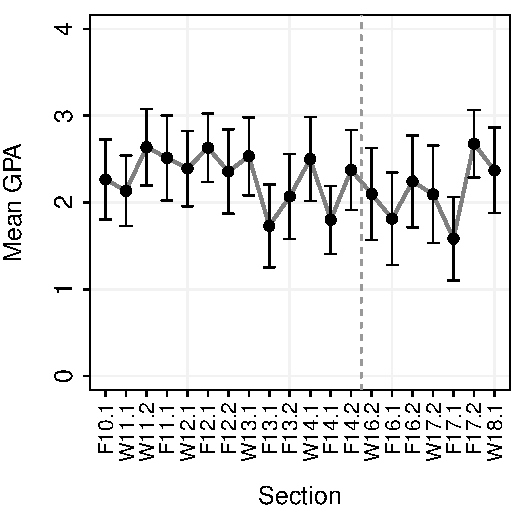
\includegraphics[width=.4\linewidth]{Figs/GradeSummary-1} 
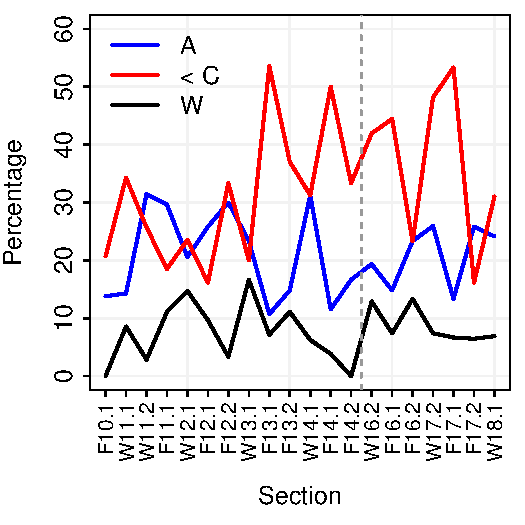
\includegraphics[width=.4\linewidth]{Figs/GradeSummary-2} 

}

\caption[Mean course GPA (with 95\% confidence intervals]{Mean course GPA (with 95\% confidence intervals; Left) and the percentage of students (Right) that earned better than an A (labeled as an ``A''), worse than a C (``< C''), or withdrew (``W'') from the course by section (abbreviated with semester (F=Fall, W=Winter), last two digits of the calendar year, and, following the period, the section number (1 or 2)). The vertical dashed line before 'W16.2' marks the shift in pedagogical approach.}\label{fig:GradeSummary}
\end{figure}


\end{knitrout}


\clearpage
\subsection{ILO \#1 (Why Statistics is Important)}
One question on the final exam asked the students to explain the importance of statistics to understanding science with explicit directions to highlight specific concepts from the course that would illustrate the student's argument. This question was meant to assess ILO \#1.

I have two goals for student achievement of this ILO. First, given that this course is required for several majors and serves as a Natural Connections course, I hoped that most students would answer this question with some broad knowledge. Second, I also hoped that the ``highest achieving'' students in the course would provide a ``very good'' answer to this foundational question. I translated these hopes into the following two goals:

\begin{Enumerate}
  \item The first quartile (the lowest 25\% of values; Q1) of proportional scores on this question would be 0.50 or better (i.e., at least half of the available points).
  \item The third quartile (the top 25\% of values; Q3) of the proportional scores on this question would be 0.90 or better.
\end{Enumerate}

\subsubsection{Results}
\vspace{-12pt}


Student achievement on this question varied substantially among sections (\tabref{tab:sumWhy}; \figref{fig:WhyBar}). The first goal was met in ten of 15 sections, including eight of the last ten sections. The second goal was met for only two of 15 sections, though it was met or nearly met in the last four sections.

\subsubsection{Actions}
\vspace{-12pt}
The course material related to this ILO was presented throughout each section, but was only explicitly discussed in the first module during the first week of each semester. While this appears to be adequate coverage to reach the lesser of the two objectives, it does not appear adequate to meet the higher objective. It should be noted that in the last two years, I provided the prompt to this question before the final exam. This did not result in appreciably higher achievement. Perhaps the prompt needs to be reconsidered. In addition, I never did develop a short mid-term assignment where students would revisit the core principles related to this ILO by finding, summarizing, and reflecting on a ``piece'' (newspaper article, journal paper, etc.) that demonstrates the importance of statistics in the student's chosen field. I did not implement this assignment as students already suggest that there is ``too much work'' in this course. Nevertheless, I will consider such an assignment for the future.
\vspace{12pt}

% latex table generated in R 3.5.0 by xtable 1.8-2 package
% Wed Jun 06 13:29:55 2018
\begin{table}[h]
\centering
\caption{Summary statistics of proportional scores on the `Why Statistics is Important' question (ILO \#1) by section (same abbreviations as in \figref{fig:GradeSummary}). Values in blue met or exceeded the objective, whereas those in red did not.} 
\label{tab:sumWhy}
\begin{tabular}{lrrrrrrrrr}
  \hline
Section & n & mean & sd & min & \textbf{Q1} & median & \textbf{Q3} & max & \% zero \\ 
  \hline
F12.1 & 28 & 0.63 & 0.18 & 0.25 & \textcolor{red}{\textcolor{blue}{0.50}} & 0.63 & \textcolor{red}{                   0.75} & 0.88 & 0.0 \\ 
  F12.2 & 26 & 0.68 & 0.26 & 0.25 & \textcolor{red}{                   0.41} & 0.69 & \textcolor{red}{                   0.88} & 1.00 & 0.0 \\ 
  W13.1 & 21 & 0.75 & 0.15 & 0.50 & \textcolor{red}{\textcolor{blue}{0.63}} & 0.75 & \textcolor{red}{                   0.88} & 1.00 & 0.0 \\ 
  F13.1 & 25 & 0.59 & 0.26 & 0.13 & \textcolor{red}{                   0.38} & 0.50 & \textcolor{red}{                   0.75} & 1.00 & 0.0 \\ 
  F13.2 & 23 & 0.61 & 0.22 & 0.25 & \textcolor{red}{                   0.38} & 0.63 & \textcolor{red}{                   0.75} & 1.00 & 0.0 \\ 
  W14.1 & 28 & 0.69 & 0.15 & 0.50 & \textcolor{red}{\textcolor{blue}{0.50}} & 0.69 & \textcolor{red}{                   0.75} & 1.00 & 0.0 \\ 
  F14.1 & 23 & 0.67 & 0.21 & 0.00 & \textcolor{red}{\textcolor{blue}{0.56}} & 0.75 & \textcolor{red}{                   0.75} & 1.00 & 4.3 \\ 
  F14.2 & 24 & 0.66 & 0.20 & 0.25 & \textcolor{red}{\textcolor{blue}{0.50}} & 0.69 & \textcolor{red}{                   0.83} & 1.00 & 0.0 \\ 
  W16.2 & 27 & 0.72 & 0.21 & 0.25 & \textcolor{red}{\textcolor{blue}{0.63}} & 0.75 & \textcolor{red}{                   0.88} & 1.00 & 0.0 \\ 
  F16.1 & 23 & 0.66 & 0.17 & 0.38 & \textcolor{red}{\textcolor{blue}{0.50}} & 0.63 & \textcolor{red}{                   0.75} & 1.00 & 0.0 \\ 
  F16.2 & 22 & 0.59 & 0.24 & 0.00 & \textcolor{red}{                   0.41} & 0.63 & \textcolor{red}{                   0.63} & 1.00 & 4.5 \\ 
  W17.2 & 24 & 0.71 & 0.23 & 0.25 & \textcolor{red}{\textcolor{blue}{0.50}} & 0.75 & \textcolor{red}{\textcolor{blue}{0.90}} & 1.00 & 0.0 \\ 
  F17.1 & 24 & 0.61 & 0.26 & 0.13 & \textcolor{red}{                   0.47} & 0.56 & \textcolor{red}{                   0.88} & 1.00 & 0.0 \\ 
  F17.2 & 28 & 0.69 & 0.26 & 0.13 & \textcolor{red}{\textcolor{blue}{0.50}} & 0.75 & \textcolor{red}{\textcolor{blue}{0.94}} & 1.00 & 0.0 \\ 
  W18.1 & 26 & 0.71 & 0.22 & 0.13 & \textcolor{red}{\textcolor{blue}{0.63}} & 0.75 & \textcolor{red}{                   0.86} & 1.00 & 0.0 \\ 
   \hline
\end{tabular}
\end{table}


\begin{knitrout}
\definecolor{shadecolor}{rgb}{0.969, 0.969, 0.969}\color{fgcolor}\begin{figure}[h]

{\centering 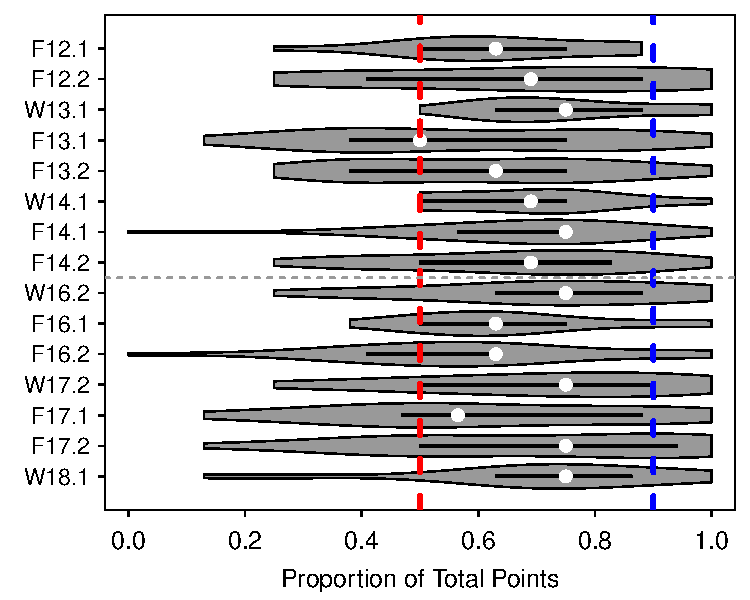
\includegraphics[width=.6\linewidth]{Figs/WhyBar-1} 

}

\caption[Violin plot (white point is the median, ends of black line are the first and third quartiles, gray polygon represents the distribution of values with thicker portions representing more students) of proportional scores on the `Why Statistics is Important' question (ILO \#1) by section (same abbreviations as in Figure 1)]{Violin plot (white point is the median, ends of black line are the first and third quartiles, gray polygon represents the distribution of values with thicker portions representing more students) of proportional scores on the `Why Statistics is Important' question (ILO \#1) by section (same abbreviations as in Figure 1). The red and blue vertical dashed lines are the goals for the Q1 and Q3 results, respectively. The horizontal dashed line before 'W16.2' marks the shift in pedagogical approach.}\label{fig:WhyBar}
\end{figure}


\end{knitrout}



\clearpage
\subsection{ILO \#8 (Two-Sample t-Test)}
One question on the final exam required students to conduct a thorough analysis of data with a ``Two-Sample t-Test.'' The question was graded with a rubric that listed the eleven steps for any hypothesis test (this rubric was supplied to the students before and during the exam). This question was intended to assess the ``two-sample quantitative'' portion of ILO \#8.

I have two goals for student achievement of this ILO. First, I hoped that most students would have gained enough knowledge to at least provide a reasonable start to an answer for this question. Second, I hoped that the majority of students would provide a ``very good'' answer to this technical question. I translated these hopes into the following two goals:

\begin{Enumerate}
  \item The first quartile (Q1) of proportional scores on this question would be 0.50 or better (i.e., 75\% of students would earn more than half of the points for this question).
  \item The median (the top 50\% of values) of proportional scores on this question would be 0.80 or better (i.e., 50\% of the students would earn more than 80\% of the points for this question).
\end{Enumerate}

\subsubsection{Results}
\vspace{-12pt}


The first goal was met in all but three section (\tabref{tab:sumT2}; \figref{fig:T2Bar}). However, the second goal was met in only four sections.

\subsubsection{Actions}
\vspace{-12pt}
This ILO was not met. A previous anecdotal content analysis suggests that many of the students are missing points on this question primarily related to properly assessing the assumptions of the method. I rewrote some of the course reading material to better emphasize this portion of the method. That does not seem to have made an appreciable difference in student achievement.
\vspace{12pt}

% latex table generated in R 3.5.0 by xtable 1.8-2 package
% Wed Jun 06 13:29:55 2018
\begin{table}[h]
\centering
\caption{Summary statistics of proportional scores on the `Two-Sample t-Test' question (ILO \#8) by section (same abbreviations as in \figref{fig:GradeSummary}). Values in blue met or exceeded the objective, whereas those in red did not.} 
\label{tab:sumT2}
\begin{tabular}{lrrrrrrrrr}
  \hline
Section & n & mean & sd & min & \textbf{Q1} & \textbf{median} & Q3 & max & \% zero \\ 
  \hline
F12.1 & 28 & 0.76 & 0.17 & 0.38 & \textcolor{red}{\textcolor{blue}{0.64}} & \textcolor{red}{                   0.76} & 0.91 & 1.00 & 0.0 \\ 
  F12.2 & 26 & 0.73 & 0.18 & 0.38 & \textcolor{red}{\textcolor{blue}{0.60}} & \textcolor{red}{                   0.74} & 0.90 & 0.94 & 0.0 \\ 
  W13.1 & 21 & 0.79 & 0.13 & 0.50 & \textcolor{red}{\textcolor{blue}{0.71}} & \textcolor{red}{\textcolor{blue}{0.82}} & 0.88 & 1.00 & 0.0 \\ 
  F13.1 & 25 & 0.52 & 0.31 & 0.00 & \textcolor{red}{                   0.32} & \textcolor{red}{                   0.44} & 0.79 & 0.97 & 12.0 \\ 
  F13.2 & 23 & 0.65 & 0.29 & 0.00 & \textcolor{red}{\textcolor{blue}{0.50}} & \textcolor{red}{                   0.76} & 0.82 & 0.97 & 4.3 \\ 
  W14.1 & 28 & 0.73 & 0.27 & 0.06 & \textcolor{red}{\textcolor{blue}{0.56}} & \textcolor{red}{\textcolor{blue}{0.84}} & 0.94 & 1.00 & 0.0 \\ 
  F14.1 & 23 & 0.62 & 0.19 & 0.15 & \textcolor{red}{\textcolor{blue}{0.52}} & \textcolor{red}{                   0.65} & 0.72 & 0.88 & 0.0 \\ 
  F14.2 & 24 & 0.63 & 0.22 & 0.12 & \textcolor{red}{\textcolor{blue}{0.53}} & \textcolor{red}{                   0.62} & 0.76 & 0.94 & 0.0 \\ 
  W16.2 & 27 & 0.61 & 0.27 & 0.00 & \textcolor{red}{\textcolor{blue}{0.50}} & \textcolor{red}{                   0.65} & 0.83 & 0.94 & 3.7 \\ 
  F16.1 & 23 & 0.60 & 0.30 & 0.00 & \textcolor{red}{\textcolor{blue}{0.50}} & \textcolor{red}{                   0.68} & 0.80 & 1.00 & 8.7 \\ 
  F16.2 & 22 & 0.75 & 0.22 & 0.12 & \textcolor{red}{\textcolor{blue}{0.71}} & \textcolor{red}{\textcolor{blue}{0.80}} & 0.90 & 0.97 & 0.0 \\ 
  W17.2 & 24 & 0.69 & 0.26 & 0.00 & \textcolor{red}{\textcolor{blue}{0.54}} & \textcolor{red}{                   0.76} & 0.91 & 0.97 & 4.2 \\ 
  F17.1 & 24 & 0.60 & 0.27 & 0.00 & \textcolor{red}{                   0.43} & \textcolor{red}{                   0.62} & 0.82 & 1.00 & 4.2 \\ 
  F17.2 & 28 & 0.80 & 0.19 & 0.38 & \textcolor{red}{\textcolor{blue}{0.72}} & \textcolor{red}{\textcolor{blue}{0.88}} & 0.95 & 1.00 & 0.0 \\ 
  W18.1 & 26 & 0.65 & 0.23 & 0.26 & \textcolor{red}{                   0.41} & \textcolor{red}{                   0.69} & 0.83 & 0.97 & 0.0 \\ 
   \hline
\end{tabular}
\end{table}


\begin{knitrout}
\definecolor{shadecolor}{rgb}{0.969, 0.969, 0.969}\color{fgcolor}\begin{figure}[h]

{\centering 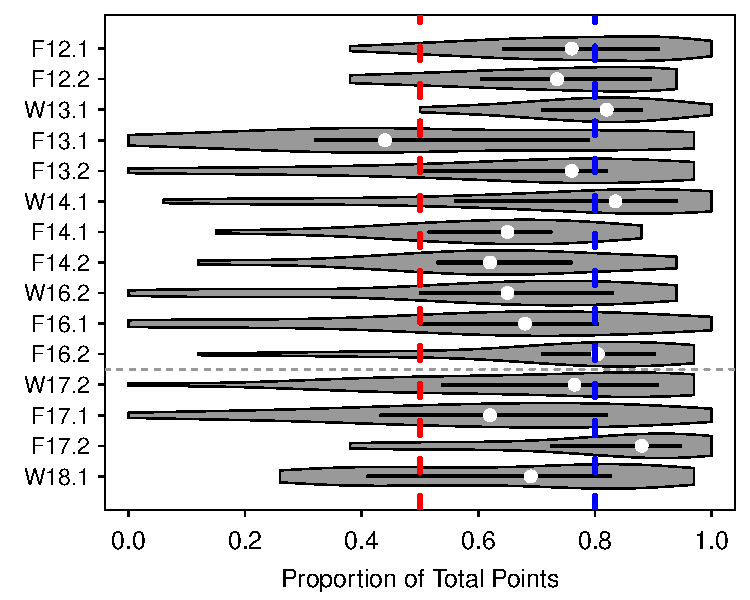
\includegraphics[width=.6\linewidth]{Figs/T2Bar-1} 

}

\caption[Violin plot (white point is the median, ends of black line are the first and third quartiles, gray polygon represents the distribution of values with thicker portions representing more students) of proportional scores on the `Two-Sample t-Test' question (part of ILO \#8) by section (same abbreviations as in Figure 1)]{Violin plot (white point is the median, ends of black line are the first and third quartiles, gray polygon represents the distribution of values with thicker portions representing more students) of proportional scores on the `Two-Sample t-Test' question (part of ILO \#8) by section (same abbreviations as in Figure 1). The red and blue vertical dashed lines are the goals for the Q1 and median results, respectively. The horizontal dashed line before 'W16.2' marks the shift in pedagogical approach.}\label{fig:T2Bar}
\end{figure}


\end{knitrout}


\clearpage
\subsection{ILO \#8 (Chi-Square Test)}
One question on the final exam required students to conduct a thorough analysis of data with a ``Chi-Square Test.''  The question was graded with a rubric that identified the eleven steps of any hypothesis test (this rubric was supplied to the students before and during the exam). This question was meant to assess the ``two-sample categorical'' portion of ILO \#8.

My two goals for student achievement of this ILO are the same as those described above for the two-sample t-test. Specifically,

\begin{Enumerate}
  \item The Q1 of proportional scores on this question will be 0.50 or better.
  \item The median of proportional scores on this question will be 0.80 or better.
\end{Enumerate}

\subsubsection{Results}
\vspace{-12pt}


Student achievement on this question has varied substantially among sections (\tabref{tab:sumChi}; \figref{fig:ChiBar}). The first goal was met in ten of the 15 sections, though there was a dip in achievement for this objective during the first two semesters of the ``flipped'' class. The second goal has only been met in seven of the 15 sections.

\subsubsection{Actions}
\vspace{-12pt}
The objectives for this ILO have not been met. In recent years, I have implemented the changes that I suggested on previous assessment reports (adjusted the course schedule to allow more time for this module and moved the final exam back so students would have more time on practice exercises at the end of the semester). While these changes are not reflected in higher achievement scores, I do think they have benefited most students. I also rewrote the reading material for this module ro make a better distinction between the chi-square and goodness-of-fit tests (and related computer code). These changes do not appear to have affected any real change in student achievement.
\vspace{12pt}

% latex table generated in R 3.5.0 by xtable 1.8-2 package
% Wed Jun 06 13:29:55 2018
\begin{table}[h]
\centering
\caption{Summary statistics of proportional scores on the `Chi-Square Test' question (ILO \#1) by section (same abbreviations as in \figref{fig:GradeSummary}). Values in blue met or exceeded the objective, whereas those in red did not.} 
\label{tab:sumChi}
\begin{tabular}{lrrrrrrrrr}
  \hline
Section & n & mean & sd & min & \textbf{Q1} & \textbf{median} & Q3 & max & \% zero \\ 
  \hline
F12.1 & 28 & 0.76 & 0.25 & 0.07 & \textcolor{red}{\textcolor{blue}{0.62}} & \textcolor{red}{\textcolor{blue}{0.82}} & 1.00 & 1.00 & 0.0 \\ 
  F12.2 & 26 & 0.72 & 0.30 & 0.00 & \textcolor{red}{\textcolor{blue}{0.62}} & \textcolor{red}{\textcolor{blue}{0.82}} & 0.97 & 1.00 & 3.8 \\ 
  W13.1 & 21 & 0.81 & 0.22 & 0.27 & \textcolor{red}{\textcolor{blue}{0.67}} & \textcolor{red}{\textcolor{blue}{0.87}} & 1.00 & 1.00 & 0.0 \\ 
  F13.1 & 25 & 0.49 & 0.32 & 0.00 & \textcolor{red}{                   0.17} & \textcolor{red}{                   0.53} & 0.77 & 1.00 & 12.0 \\ 
  F13.2 & 23 & 0.64 & 0.27 & 0.00 & \textcolor{red}{                   0.45} & \textcolor{red}{                   0.73} & 0.82 & 1.00 & 4.3 \\ 
  W14.1 & 28 & 0.72 & 0.32 & 0.00 & \textcolor{red}{\textcolor{blue}{0.58}} & \textcolor{red}{\textcolor{blue}{0.87}} & 1.00 & 1.00 & 7.1 \\ 
  F14.1 & 23 & 0.70 & 0.22 & 0.13 & \textcolor{red}{\textcolor{blue}{0.58}} & \textcolor{red}{                   0.73} & 0.87 & 1.00 & 0.0 \\ 
  F14.2 & 24 & 0.75 & 0.25 & 0.13 & \textcolor{red}{\textcolor{blue}{0.69}} & \textcolor{red}{\textcolor{blue}{0.80}} & 0.93 & 1.00 & 0.0 \\ 
  W16.2 & 27 & 0.61 & 0.31 & 0.00 & \textcolor{red}{                   0.45} & \textcolor{red}{                   0.67} & 0.88 & 1.00 & 7.4 \\ 
  F16.1 & 23 & 0.61 & 0.34 & 0.00 & \textcolor{red}{                   0.32} & \textcolor{red}{                   0.77} & 0.85 & 1.00 & 8.7 \\ 
  F16.2 & 22 & 0.82 & 0.23 & 0.00 & \textcolor{red}{\textcolor{blue}{0.78}} & \textcolor{red}{\textcolor{blue}{0.90}} & 0.99 & 1.00 & 4.5 \\ 
  W17.2 & 24 & 0.66 & 0.25 & 0.00 & \textcolor{red}{\textcolor{blue}{0.57}} & \textcolor{red}{                   0.72} & 0.83 & 1.00 & 4.2 \\ 
  F17.1 & 24 & 0.60 & 0.31 & 0.00 & \textcolor{red}{                   0.44} & \textcolor{red}{                    0.6} & 0.88 & 1.00 & 4.2 \\ 
  F17.2 & 28 & 0.78 & 0.20 & 0.33 & \textcolor{red}{\textcolor{blue}{0.63}} & \textcolor{red}{\textcolor{blue}{0.87}} & 0.93 & 1.00 & 0.0 \\ 
  W18.1 & 26 & 0.69 & 0.26 & 0.07 & \textcolor{red}{\textcolor{blue}{0.53}} & \textcolor{red}{                   0.73} & 0.92 & 1.00 & 0.0 \\ 
   \hline
\end{tabular}
\end{table}


\begin{knitrout}
\definecolor{shadecolor}{rgb}{0.969, 0.969, 0.969}\color{fgcolor}\begin{figure}[h]

{\centering 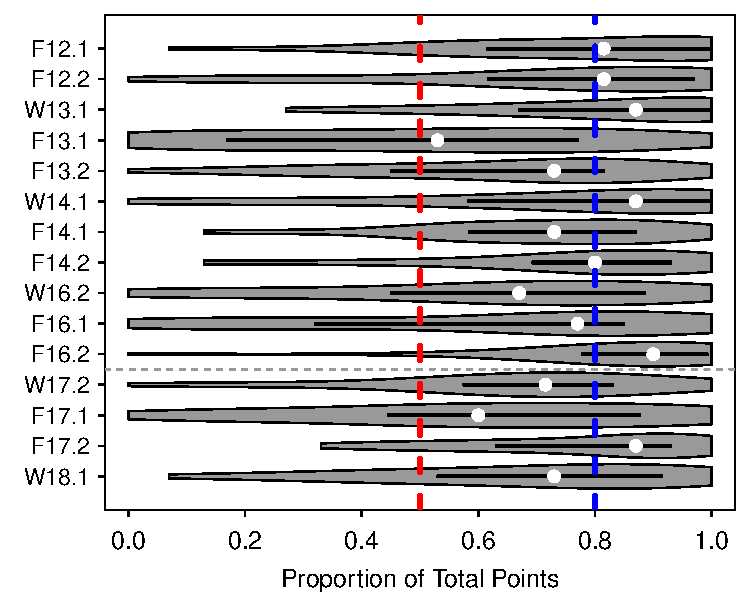
\includegraphics[width=.6\linewidth]{Figs/ChiBar-1} 

}

\caption[Violin plot (white point is the median, ends of black line are the first and third quartiles, gray polygon represents the distribution of values with thicker portions representing more students) of proportional scores on the `Chi-Square Test' question (part of ILO \#8) by section (same abbreviations as in Figure 1]{Violin plot (white point is the median, ends of black line are the first and third quartiles, gray polygon represents the distribution of values with thicker portions representing more students) of proportional scores on the `Chi-Square Test' question (part of ILO \#8) by section (same abbreviations as in Figure 1. The red and blue vertical dashed lines are the goals for the Q1 and median, respectively. The horizontal dashed line before 'W16.2' marks the shift in pedagogical approach.}\label{fig:ChiBar}
\end{figure}


\end{knitrout}


\clearpage
\subsection{ILO \#3 (Exploratory Data Analysis)}
Three questions on the final exam required students to conduct exploratory data analyses (EDA). The analyses below assess their univariate and bivariate EDAs for quantitative data. The univariate EDA for categorical data is not assessed (it is only a two point question that does not provide much useful information).

As this is fairly easy material that is foundational to all statistical analyses, I hoped that most student would perform well on these questions. I also expected most ``high achieving'' students to provide very strong answers to these questions. I translated these hopes into the following two goals (for each of the univariate and bivariate questions):

\begin{Enumerate}
  \item The Q1 of proportional scores on this question will be 0.7 or better (i.e., 75\% of the students will earn 70\% or more of the points for this question).
  \item The median of proportional scores on this question will be 0.9 or better (i.e., at least half of the students will earn 90\% or more of the points for this question).
\end{Enumerate}

\subsubsection{Results}
\vspace{-12pt}

The first goal for the univariate EDA was met in only five of 15 sections, with less success and considerable variability in recent sections (\tabref{tab:sumUEDAQ}; \figref{fig:UEDAQBar}). The second goal was met more often, having been met in eight of 15 sections. This suggests many students perform well on this question, but those that do not really do not do well. Anecdotal content analysis suggests that many students forget to identify why they chose to use the median and IQR or mean and SD as their measures of center and dispersion. Failing to do this results in a loss of 20\% for this question. If most students were to do this (and do it correctly), the results in \tabref{tab:sumUEDAQ} suggest that the objectives would then be met.

The first goal for the bivariate EDA was met in only four of 15 sections, with less success and considerable variability in recent sections (\tabref{tab:sumBEDAQ}; \figref{fig:BEDAQBar}). The second goal was met even less frequently, having been met in only one of 15 sections. Anecdotal content analysis suggests that many students forget to identify whether or not (and why) they used the correlation coefficient to assess the strength of relationship. Failing to do this results in a loss of 20\% for this question. If most students were to do this (and do it correctly), the results in \tabref{tab:sumBEDAQ} suggest that the objectives would then be met.

\subsubsection{Actions}
\vspace{-12pt}
The objectives for these two portions of this ILO were largely not met. However, anecdotal content analysis suggests that students perform fairly well on the main components of this question (i.e., describing four aspects of the EDA), but often fail to explain why they did or did not use certain statistics in their descriptions. When I rewrote the readings for these sections last year, I emphasized the importance of these items in performing the EDA. These changes do not appear to have affected any realy change in student achievement.
\vspace{12pt}

% latex table generated in R 3.5.0 by xtable 1.8-2 package
% Wed Jun 06 13:29:55 2018
\begin{table}[h]
\centering
\caption{Summary statistics of proportional scores on the `univariate EDA' question (ILO \#3) by section (same abbreviations as in \figref{fig:GradeSummary}). Values in blue met or exceeded the objective, whereas those in red did not.} 
\label{tab:sumUEDAQ}
\begin{tabular}{lrrrrrrrrr}
  \hline
Section & n & mean & sd & min & \textbf{Q1} & \textbf{median} & Q3 & max & \% zero \\ 
  \hline
F12.1 & 28 & 0.82 & 0.27 & 0.00 & \textcolor{red}{\textcolor{blue}{0.80}} & \textcolor{red}{\textcolor{blue}{0.95}} & 1.00 & 1.00 & 3.6 \\ 
  F12.2 & 26 & 0.77 & 0.28 & 0.00 & \textcolor{red}{\textcolor{blue}{0.70}} & \textcolor{red}{                    0.8} & 1.00 & 1.00 & 3.8 \\ 
  W13.1 & 21 & 0.86 & 0.19 & 0.40 & \textcolor{red}{\textcolor{blue}{0.80}} & \textcolor{red}{\textcolor{blue}{1.00}} & 1.00 & 1.00 & 0.0 \\ 
  F13.1 & 25 & 0.79 & 0.30 & 0.00 & \textcolor{red}{                    0.6} & \textcolor{red}{\textcolor{blue}{1.00}} & 1.00 & 1.00 & 4.0 \\ 
  F13.2 & 23 & 0.74 & 0.28 & 0.00 & \textcolor{red}{                   0.55} & \textcolor{red}{                    0.8} & 1.00 & 1.00 & 4.3 \\ 
  W14.1 & 28 & 0.74 & 0.32 & 0.00 & \textcolor{red}{                    0.6} & \textcolor{red}{                    0.8} & 1.00 & 1.00 & 7.1 \\ 
  F14.1 & 23 & 0.69 & 0.33 & 0.00 & \textcolor{red}{                   0.45} & \textcolor{red}{                    0.8} & 1.00 & 1.00 & 8.7 \\ 
  F14.2 & 24 & 0.82 & 0.21 & 0.40 & \textcolor{red}{                    0.6} & \textcolor{red}{\textcolor{blue}{0.90}} & 1.00 & 1.00 & 0.0 \\ 
  W16.2 & 27 & 0.74 & 0.23 & 0.20 & \textcolor{red}{                    0.6} & \textcolor{red}{                    0.8} & 0.90 & 1.00 & 0.0 \\ 
  F16.1 & 23 & 0.70 & 0.34 & 0.00 & \textcolor{red}{                   0.45} & \textcolor{red}{                    0.8} & 1.00 & 1.00 & 4.3 \\ 
  F16.2 & 22 & 0.86 & 0.18 & 0.40 & \textcolor{red}{\textcolor{blue}{0.72}} & \textcolor{red}{\textcolor{blue}{1.00}} & 1.00 & 1.00 & 0.0 \\ 
  W17.2 & 24 & 0.75 & 0.32 & 0.00 & \textcolor{red}{                   0.55} & \textcolor{red}{\textcolor{blue}{0.90}} & 1.00 & 1.00 & 4.2 \\ 
  F17.1 & 24 & 0.78 & 0.22 & 0.30 & \textcolor{red}{                    0.6} & \textcolor{red}{                   0.85} & 1.00 & 1.00 & 0.0 \\ 
  F17.2 & 28 & 0.89 & 0.15 & 0.30 & \textcolor{red}{\textcolor{blue}{0.80}} & \textcolor{red}{\textcolor{blue}{0.90}} & 1.00 & 1.00 & 0.0 \\ 
  W18.1 & 26 & 0.78 & 0.31 & 0.00 & \textcolor{red}{                   0.62} & \textcolor{red}{\textcolor{blue}{1.00}} & 1.00 & 1.00 & 3.8 \\ 
   \hline
\end{tabular}
\end{table}


% latex table generated in R 3.5.0 by xtable 1.8-2 package
% Wed Jun 06 13:29:55 2018
\begin{table}[h]
\centering
\caption{Summary statistics of proportional scores on the `bivariate EDA' question (ILO \#3) by section (same abbreviations as in \figref{fig:GradeSummary}). Values in blue met or exceeded the objective, whereas those in red did not.} 
\label{tab:sumBEDAQ}
\begin{tabular}{lrrrrrrrrr}
  \hline
Section & n & mean & sd & min & \textbf{Q1} & \textbf{median} & Q3 & max & \% zero \\ 
  \hline
F12.1 & 28 & 0.76 & 0.27 & 0.00 & \textcolor{red}{\textcolor{blue}{0.75}} & \textcolor{red}{                    0.8} & 0.92 & 1.00 & 7.1 \\ 
  F12.2 & 26 & 0.80 & 0.31 & 0.00 & \textcolor{red}{\textcolor{blue}{0.80}} & \textcolor{red}{\textcolor{blue}{0.90}} & 1.00 & 1.00 & 11.5 \\ 
  W13.1 & 21 & 0.67 & 0.30 & 0.00 & \textcolor{red}{                    0.5} & \textcolor{red}{                    0.7} & 1.00 & 1.00 & 4.8 \\ 
  F13.1 & 25 & 0.72 & 0.30 & 0.00 & \textcolor{red}{\textcolor{blue}{0.70}} & \textcolor{red}{                    0.8} & 0.80 & 1.00 & 12.0 \\ 
  F13.2 & 23 & 0.70 & 0.18 & 0.30 & \textcolor{red}{                   0.65} & \textcolor{red}{                    0.7} & 0.80 & 1.00 & 0.0 \\ 
  W14.1 & 28 & 0.78 & 0.22 & 0.20 & \textcolor{red}{                    0.6} & \textcolor{red}{                    0.8} & 1.00 & 1.00 & 0.0 \\ 
  F14.1 & 23 & 0.62 & 0.32 & 0.00 & \textcolor{red}{                   0.45} & \textcolor{red}{                    0.7} & 0.80 & 1.00 & 13.0 \\ 
  F14.2 & 24 & 0.67 & 0.28 & 0.00 & \textcolor{red}{                    0.5} & \textcolor{red}{                    0.7} & 0.90 & 1.00 & 4.2 \\ 
  W16.2 & 27 & 0.62 & 0.28 & 0.00 & \textcolor{red}{                    0.5} & \textcolor{red}{                    0.7} & 0.80 & 1.00 & 7.4 \\ 
  F16.1 & 23 & 0.64 & 0.32 & 0.00 & \textcolor{red}{                   0.45} & \textcolor{red}{                    0.8} & 0.80 & 1.00 & 8.7 \\ 
  F16.2 & 22 & 0.73 & 0.30 & 0.00 & \textcolor{red}{                   0.62} & \textcolor{red}{                    0.8} & 0.90 & 1.00 & 9.1 \\ 
  W17.2 & 24 & 0.67 & 0.37 & 0.00 & \textcolor{red}{                    0.6} & \textcolor{red}{                   0.85} & 0.90 & 1.00 & 20.8 \\ 
  F17.1 & 24 & 0.59 & 0.34 & 0.00 & \textcolor{red}{                    0.4} & \textcolor{red}{                    0.6} & 0.80 & 1.00 & 16.7 \\ 
  F17.2 & 28 & 0.79 & 0.18 & 0.20 & \textcolor{red}{\textcolor{blue}{0.70}} & \textcolor{red}{                    0.8} & 0.90 & 1.00 & 0.0 \\ 
  W18.1 & 26 & 0.49 & 0.34 & 0.00 & \textcolor{red}{                    0.2} & \textcolor{red}{                   0.55} & 0.70 & 1.00 & 15.4 \\ 
   \hline
\end{tabular}
\end{table}


\begin{knitrout}
\definecolor{shadecolor}{rgb}{0.969, 0.969, 0.969}\color{fgcolor}\begin{figure}[h]

{\centering 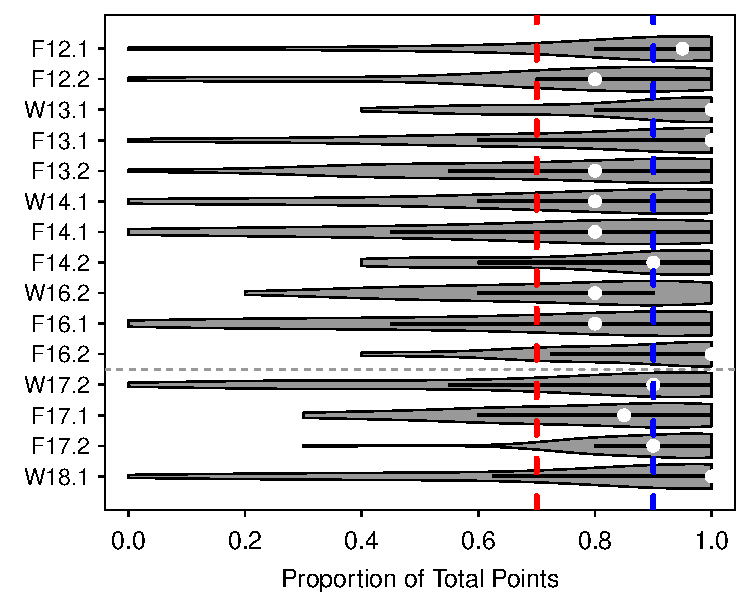
\includegraphics[width=.6\linewidth]{Figs/UEDAQBar-1} 

}

\caption[Violin plot (white point is the median, ends of black line are the first and third quartiles, gray polygon represents the distribution of values with thicker portions representing more students) of proportional scores on the `univariate EDA' question (part of ILO \#3) by section (same abbreviations as in Figure 1)]{Violin plot (white point is the median, ends of black line are the first and third quartiles, gray polygon represents the distribution of values with thicker portions representing more students) of proportional scores on the `univariate EDA' question (part of ILO \#3) by section (same abbreviations as in Figure 1). The red and blue vertical dashed lines are the goals for the Q1 and median, respectively. The horizontal dashed line before 'W16.2' marks the shift in pedagogical approach.}\label{fig:UEDAQBar}
\end{figure}


\end{knitrout}

\begin{knitrout}
\definecolor{shadecolor}{rgb}{0.969, 0.969, 0.969}\color{fgcolor}\begin{figure}[h]

{\centering 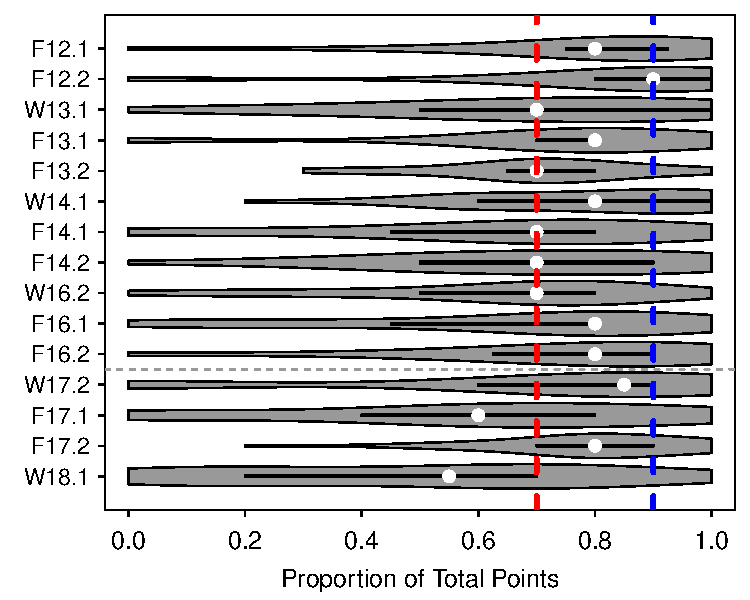
\includegraphics[width=.6\linewidth]{Figs/BEDAQBar-1} 

}

\caption[Violin plot (white point is the median, ends of black line are the first and third quartiles, gray polygon represents the distribution of values with thicker portions representing more students) of proportional scores on the `bivariate EDA' question (part of ILO \#3) by section (same abbreviations as in Figure 1)]{Violin plot (white point is the median, ends of black line are the first and third quartiles, gray polygon represents the distribution of values with thicker portions representing more students) of proportional scores on the `bivariate EDA' question (part of ILO \#3) by section (same abbreviations as in Figure 1). The red and blue vertical dashed lines are the goals for the Q1 and median, respectively. The horizontal dashed line before 'W16.2' marks the shift in pedagogical approach.}\label{fig:BEDAQBar}
\end{figure}


\end{knitrout}



\clearpage
\subsection{ILO \#4 (Linear Regression)}
Three questions on the final exam required students to answer questions from linear regression results. Scores on these three questions were summed to provide an overall assessment of the student's ability to apply linear regression results.

Linear regression is a foundational statistical method in nearly all fields of study. Therefore, I hoped that most student would perform well on these questions. I also would like to see most ``high achieving'' students provide very strong answers to these questions. I translated these hopes into the following two goals:

\begin{Enumerate}
  \item The Q1 of proportional scores on this question will be 0.5 or better.
  \item The median of proportional scores on this question will be 0.9 or better.
\end{Enumerate}

\subsubsection{Results}
\vspace{-12pt}


Student achievement on the univariate EDA question varied substantially \figrefp{fig:RegBar} and only the first goal was met by only one section. In fact, the first goal was NOT met at the median (rather than Q1) and the second goal was NOT met at Q3 (rather than the median) in many sections. Furthermore, many sections had more than 10\%, with some sections approaching 25\%, of the students that did not earn any points on this question. These results suggest very poor overall achievement on this ILO.

\subsubsection{Actions}
\vspace{-12pt}
In previous assessments, I noted that students need more practice with this material. In the ``flipped'' class, they did get more practice so, perhaps, the quality of that practice, rather than the quantity, is the problem. I will reconsider the class exercises, review questions in the reading, and the homework problems to potentially address this finding. In the previous assessment, I also questioned whether these three questions are an adequate assessment of the students' understanding of this material. While that may be an issue, these three questions are consistent with questions asked on the class exercises, review exercises, and homework problems.
\vspace{12pt}

% latex table generated in R 3.5.0 by xtable 1.8-2 package
% Wed Jun 06 13:29:55 2018
\begin{table}[h]
\centering
\caption{Summary statistics of proportional scores on the `linear regression' question (ILO \#4) by section (same abbreviations as in \figref{fig:GradeSummary}). Values in blue met or exceeded the objective, whereas those in red did not.} 
\label{tab:sumReg}
\begin{tabular}{lrrrrrrrrr}
  \hline
Section & n & mean & sd & min & \textbf{Q1} & \textbf{median} & Q3 & max & \% zero \\ 
  \hline
F12.1 & 28 & 0.63 & 0.30 & 0.00 & \textcolor{red}{                    0.4} & \textcolor{red}{0.67} & 0.94 & 1.00 & 7.1 \\ 
  F12.2 & 26 & 0.64 & 0.29 & 0.17 & \textcolor{red}{                   0.42} & \textcolor{red}{0.62} & 0.92 & 1.00 & 0.0 \\ 
  W13.1 & 21 & 0.60 & 0.29 & 0.00 & \textcolor{red}{                   0.33} & \textcolor{red}{0.67} & 0.92 & 1.00 & 4.8 \\ 
  F13.1 & 25 & 0.40 & 0.33 & 0.00 & \textcolor{red}{                   0.17} & \textcolor{red}{0.33} & 0.67 & 1.00 & 24.0 \\ 
  F13.2 & 23 & 0.50 & 0.38 & 0.00 & \textcolor{red}{                   0.17} & \textcolor{red}{ 0.5} & 0.83 & 1.00 & 21.7 \\ 
  W14.1 & 28 & 0.66 & 0.35 & 0.00 & \textcolor{red}{                   0.46} & \textcolor{red}{0.67} & 0.94 & 1.00 & 14.3 \\ 
  F14.1 & 23 & 0.46 & 0.36 & 0.00 & \textcolor{red}{                   0.04} & \textcolor{red}{0.58} & 0.71 & 1.00 & 26.1 \\ 
  F14.2 & 24 & 0.44 & 0.31 & 0.00 & \textcolor{red}{                   0.31} & \textcolor{red}{0.42} & 0.60 & 1.00 & 20.8 \\ 
  W16.2 & 27 & 0.53 & 0.34 & 0.00 & \textcolor{red}{                   0.25} & \textcolor{red}{0.58} & 0.79 & 1.00 & 14.8 \\ 
  F16.1 & 23 & 0.53 & 0.35 & 0.00 & \textcolor{red}{                   0.33} & \textcolor{red}{0.42} & 0.92 & 1.00 & 8.7 \\ 
  F16.2 & 22 & 0.67 & 0.33 & 0.00 & \textcolor{red}{                   0.39} & \textcolor{red}{0.79} & 0.92 & 1.00 & 9.1 \\ 
  W17.2 & 24 & 0.52 & 0.36 & 0.00 & \textcolor{red}{                   0.29} & \textcolor{red}{ 0.5} & 0.85 & 1.00 & 16.7 \\ 
  F17.1 & 24 & 0.52 & 0.34 & 0.00 & \textcolor{red}{                   0.33} & \textcolor{red}{0.58} & 0.69 & 1.00 & 16.7 \\ 
  F17.2 & 28 & 0.70 & 0.27 & 0.00 & \textcolor{red}{\textcolor{blue}{0.58}} & \textcolor{red}{0.79} & 0.92 & 1.00 & 7.1 \\ 
  W18.1 & 26 & 0.49 & 0.33 & 0.00 & \textcolor{red}{                   0.33} & \textcolor{red}{ 0.5} & 0.75 & 1.00 & 15.4 \\ 
   \hline
\end{tabular}
\end{table}


\begin{knitrout}
\definecolor{shadecolor}{rgb}{0.969, 0.969, 0.969}\color{fgcolor}\begin{figure}[h]

{\centering 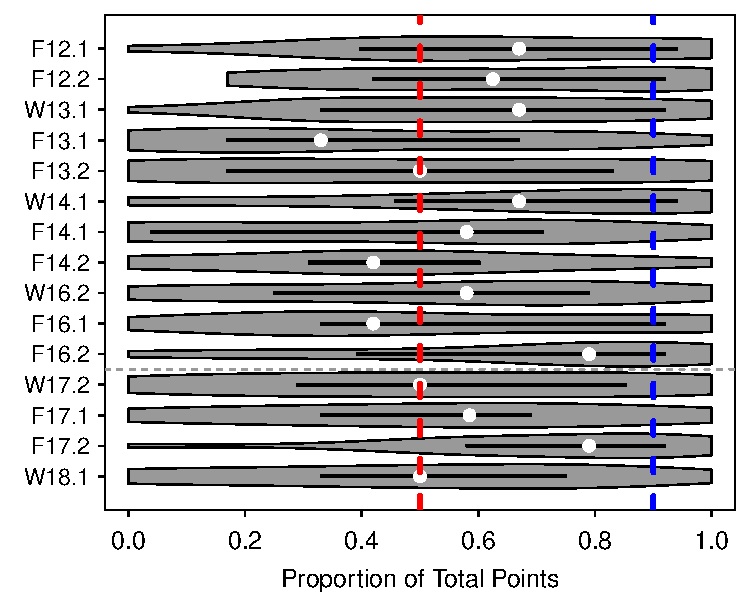
\includegraphics[width=.6\linewidth]{Figs/RegBar-1} 

}

\caption[Violin plot (white point is the median, ends of black line are the first and third quartiles, gray polygon represents the distribution of values with thicker portions representing more students) of proportional scores on the `linear regression' question (part of ILO \#4) by section (same abbreviations as in Figure 1)]{Violin plot (white point is the median, ends of black line are the first and third quartiles, gray polygon represents the distribution of values with thicker portions representing more students) of proportional scores on the `linear regression' question (part of ILO \#4) by section (same abbreviations as in Figure 1). The red and blue vertical dashed lines are the goals for the Q1 and median, respectively. The horizontal dashed line before 'W16.2' marks the shift in pedagogical approach.}\label{fig:RegBar}
\end{figure}


\end{knitrout}



\clearpage
\section{Overall Thoughts}
Overall, it does not appear that any pedagogical changes that I make to this class results in any sort of sustained improvement in student achievement or learning. For the last three academic years I have taught this course as a ``flipped'' course where students largely prepare outside of class and then work on class exercises and ask me questions during class periods. There is no evidence that this approach has led to an increase (or a decrease) in student learning (at least on the ILOs that I have assessed).

I think that there are a variety of possible reasons for this finding. First, it appears to me that many students do not fully engage outside of the class with the material provided to prepare for class. View counters on the videos that I control (I have videos on Vimeo that I have made, but I also use videos on YouTube that I have not made) suggest that very few students have watched these videos (and even fewer have watched them in their entirety). There is some evidence that students have engaged with the reading material (i.e., they can use their reading notes on the daily quizzes), but anecdotal observations suggest that that interaction is superficial at best for most students.

Second, many students do not seem to take full advantage of the opportunity to ask me questions during the class period. This may be due in part to their lack of preparation for the class period (see previous paragraph). However, this may also be because students find me intimidating. I attempted to address the ``intimidation'' problem in W17 (and after) by requiring students to come visit with me during office hours during the first two weeks of the course. While I think that this is a good idea, it did not seem to open channels of communication in general. Finally, some students did not take the class time seriously. In other words, without a professor ``lecturing'' they would often distract themselves with their phones, the computers, or other things, or would simple leave class early. I attempted to address some of these issues in W17 by banning ``devices'' and implementing a participation portion to their grade that was primarily based on staying focused during class. I believe that these policy changes helped with the class, but they did not seem to increase student achievement or learning.

Third, many students did not take advantage of out-of-class resources such as my office hours or tutoring sessions. Students in F16 used the tutors more (by my recollection) than in any other recent semester. However, students in W17 were exactly opposite. In addition, very few students sought help from me during my office hours.

I do believe that the ``flipped'' structure is appropriate for this type of class (i.e., the basic concepts can be learned from readings and videos and then augmented and cemented by practicing and extending what was learned with access to the professor). Thus, I plan to continue this structure for at least the next year.

For Fall 2018, I made the changes in the reading materials that I suggested in my last assessment report (I removed some of the items in the readings that make it easy for students to skim over the material and prepared a ``Preparation Guide'' for each module that required students to actually read the readings and watch the videos to answer the questions on the guide).

Future assessments will continue to monitor student achievement on these five ILOs. In addition, I will develop analyses to assess student achievement on other ILOs.

\cleardoublepage
\phantomsection
\section*{Reproducibility Information}
 \addcontentsline{toc}{section}{Reproducibility Information}
\begin{Itemize}
  \item \textbf{Compiled Date:} Wed Jun 06 2018
  \item \textbf{Compiled Time:} 1:29:58 PM
  \item \textbf{Code Execution Time:} 1.77 s
  \item \textbf{R Version:} R version 3.5.0 (2018-04-23)
  \item \textbf{System:} Windows, i386-w64-mingw32/i386 (32-bit)
  \item \textbf{Base Packages:} base, datasets, graphics, grDevices, methods, stats, utils
  \item \textbf{Required Packages:} FSA, readxl, xtable, magrittr, dplyr, knitr, vioplot, plotrix and their dependencies (assertthat, bindrcpp, car, cellranger, dunn.test, epitools, evaluate, glue, gplots, graphics, grDevices, highr, lmtest, markdown, methods, pkgconfig, plyr, R6, Rcpp, rlang, sciplot, sm, stats, stringr, tibble, tidyselect, tools, utils, yaml)
  \item \textbf{Other Packages:} bindrcpp\_0.2.2, dplyr\_0.7.5, FSA\_0.8.20.9000, knitr\_1.20, magrittr\_1.5, plotrix\_3.7-2, readxl\_1.1.0, sm\_2.2-5.5, vioplot\_0.2, xtable\_1.8-2
  \item \textbf{Loaded-Only Packages:} assertthat\_0.2.0, bindr\_0.1.1, cellranger\_1.1.0, compiler\_3.5.0, evaluate\_0.10.1, glue\_1.2.0, pillar\_1.2.3, pkgconfig\_2.0.1, plyr\_1.8.4, purrr\_0.2.5, R6\_2.2.2, Rcpp\_0.12.17, rlang\_0.2.1, stringi\_1.1.7, stringr\_1.3.1, tcltk\_3.5.0, tibble\_1.4.2, tidyselect\_0.2.4, tools\_3.5.0
\end{Itemize}



\end{document}
